\documentclass[12pt]{article}
\usepackage{amsmath}
\usepackage{amssymb}
\usepackage{graphicx}
\usepackage{hyperref}
\usepackage{multicol}
\usepackage[latin1]{inputenc}
\usepackage{listings}
\usepackage{scrextend}


% Used for code blocks ----------------------------------------------------------------
\usepackage{color}
\usepackage{xcolor}
\usepackage{listings}

\usepackage{caption}
\DeclareCaptionFont{white}{\color{white}}
\DeclareCaptionFormat{listing}{\colorbox{gray}{\parbox{\textwidth}{#1#2#3}}}
\captionsetup[lstlisting]{format=listing,labelfont=white,textfont=white}
% -----------------------------------------------------------------------------------------



\title{ComS 342\\Recitation 2, 10:00 Tuesday\\Homework 2}
\author{Sean Gordon}
%\date{09/09/2019}

\begin{document}
\maketitle


1)\begin{multicols}{2}
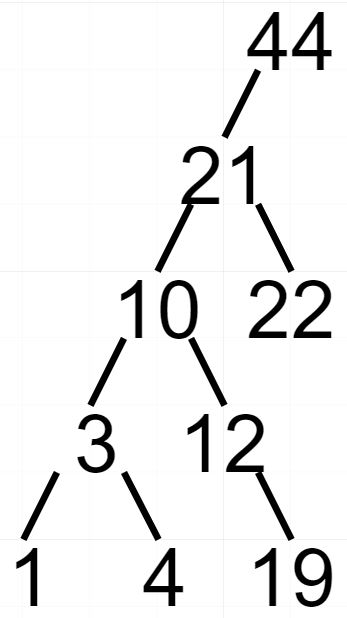
\includegraphics[scale=.4]{HW2_Pt1a}\\
\columnbreak
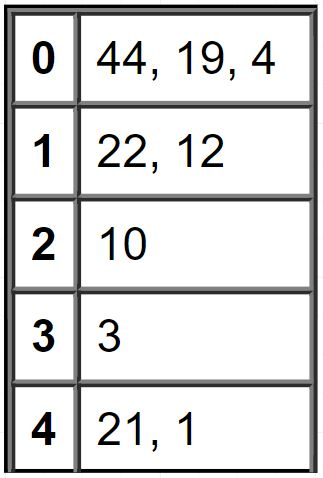
\includegraphics[scale=.5]{HW2_Pt1b}\\
\end{multicols} 

\noindent 2a)
\begin{lstlisting}[label=some-code]
succ(H, x){

    int succ = H[0]
    
    for(int i=1; i < H.length; i++){
        if(H[i] > x && H[i] < succ){
            succ = H[i]
        }
    }
    
    return succ
}
	
\end{lstlisting}
As there is only one for loop from 1 to n, runtime = O(n).\\\\

\noindent b) As there is one for loop from 0 to n containing succ() which runs O(n), this algorithm runs in O($n^2$) time.
\begin{lstlisting}[label=some-code]
better(H){
    
    n = number of elements in H
    arr = new array of length n
    
    //Copy H into arr (O(n)):
    for (index, key in H)
    	arr[index] = key

    //Sort arr (O(log(n))):
    mergeSort(arr)
    
    return arr
}
\end{lstlisting}
This algorithm runs in O(n) time.
\pagebreak

\noindent 3)
\begin{lstlisting}[label=some-code]
isUndirected(G){
    
    Make hashtable H with hash function `val % G.length'
    
    for (k = 0 to G.length){
        pair = G[k]
        
        //Add a `tally' to both vertices involved
        H[i] = j
        H[j] = i
    }
    
    for(k = 0 to H.length){
        arr = H[k]
        
        //If there aren't an even # of entries
        if( arr.length % 2 != 0)
            return false
    }
    
    return true
}
\end{lstlisting}
This algorithm runs in O(n) time.
\pagebreak

\noindent 4a)
%\begin{lstlisting}[label=some-code,caption=Some Code]
\begin{lstlisting}[label=some-code]
decreaseKey(index, delta) {
    H[index] = H[index] - delta
    
    while( H[index] > current parent ){
    	index2 = current parent index
    	swap H[index] and (current parent)
    	index = index2 
    }
}
\end{lstlisting}

\noindent b) As it was not specified (thanks for that), I will be assuming we are conforming to average case time complexity.\\
An $\bold{average\ case}$ time complexity of O(1) for $findKey(v)$ can be acheived using a $hash\ table$ with a $hash\ function$ that allows a sufficiently large maximum index value (1000, maybe) so that conflicts are rare.\\
The process is explained below:\\

\noindent $\bold{Adding\ to\ hash\ table:}$\\
Every time a value $val$ is added to the $minheap$, it will be added to the $hash\ table$ as well.\\
Value $val$ will be put through the $hash\ function$ to find the $hash\ table\ index$.\\
The item actually inserted into the $hash\ table$ will be an object containing $val$ and $val$'s index in the $minheap$ (not the above index).\\

\noindent $\bold{Finding\ index\ of\ k:}$\\
The given value $k$ will then be put through the $hash\ function$, resulting in index $i$.\\
The contents of the $hash\ table$ at $i$ will be parsed through to find the object with the value of $k$, and thus its $index$.\\
In the $\bold{average\ case}$ this search will take O(1) time, as there will likely be very few entries at that index.

\end{document}